%----------------------------------------------------------------------------
\chapter{Áttekintés}
\label{sec:overview}
%----------------------------------------------------------------------------
\section{A perifériaillesztő modul felépítése}
%----------------------------------------------------------------------------

% \begin{center}
%     \begin{tikzpicture}
%         \tikzset{
%             top/.style= {draw, rectangle, inner sep=20pt, minimum height=0.6\textwidth, minimum width=0.8\textwidth, align=center},
%             module/.style= {draw, rectangle, minimum height=0.5\textwidth ,minimum width=0.3\textwidth},
%             input/.style  = {coordinate},
%             output/.style = {coordinate}}
%         \node[input] (PCLK) at (-0.55\textwidth, 0.21875\textwidth) {};
%         \node[input] (PRESETn) at (-0.55\textwidth, 0.15625\textwidth) {};
%         \node[input] (PADDR) at (-0.55\textwidth, -0.09375\textwidth) {};
%         \node[input] (PSELx) at (-0.55\textwidth, 0.03125\textwidth) {};
%         \node[input] (PENABLE) at (-0.55\textwidth, -0.03125\textwidth) {};
%         \node[input] (PWRITE) at (-0.55\textwidth, -0.09375\textwidth) {};
%         \node[input] (PRDATA) at (-0.55\textwidth, -0.15625\textwidth) {};
%         \node[input] (PWDATA) at (-0.55\textwidth, -0.21875\textwidth) {};
%         \node[output] (SCL) at (0.55\textwidth, 0) {};
%         \node[module] (APB) at (-0.3\textwidth, 0) {};
%         \node[above left] at (APB.south east) {mod\_apb};
%         \draw[->] (PCLK) -- node[auto] {PCLK} (APB.west);
%         \draw[->] (PRESETn) -- node[auto] {PRESETn} (APB.west);
%         \draw[->] (PADDR) -- node[auto] {PADDR} (APB.west);
%         \draw[->] (PSELx) -- node[auto] {PSELx} (APB.west);
%         \draw[->] (PENABLE) -- node[auto] {PENABLE} (APB.west);
%         \draw[->] (PWRITE) -- node[auto] {PWRITE} (APB.west);
%         \draw[->] (PRDATA) -- node[auto] {PRDATA} (APB.west);
%         \node[module] (I2C) at (0.3\textwidth, 0) {};
%         \node[above left] at (I2C.south east) {mod\_i2c};
%         \draw[->] (I2C.east) -- node[auto] {SCL} (SCL);
%         \node[top, fit=(APB)(I2C)] (TOP) at (0,0) {};
%         \node[above left] at (TOP.south east) {mod\_top};
%         % \node[]
%     \end{tikzpicture}
% \end{center}
Mint az a \figref{modtop} ábrán is látszik, modulunk (\emph{mod\_top}) 2 almodult tartalmaz, a feladatkíírásnak megfelelően: egy \emph{mod\_apb} modulból, ami közvetlenül az APB buszra csatlakozik, és egy \emph{mod\_i2c} modulból, ami a soros kommunkáció vonalaival van összeköttetésben.

\begin{figure}[ht!]
    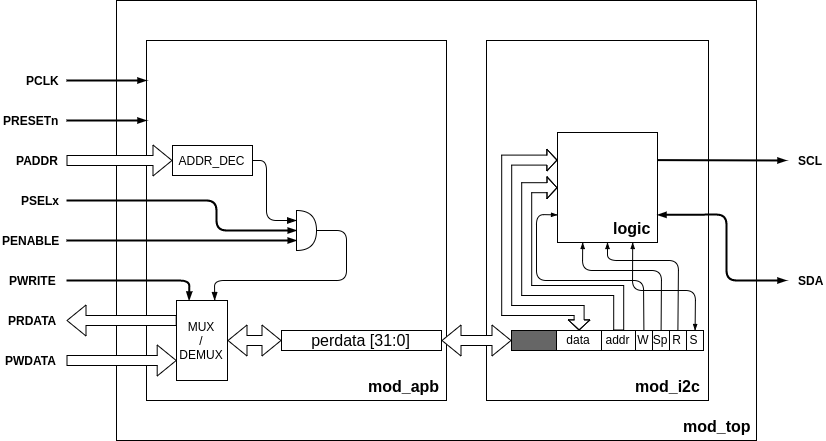
\includegraphics[width=\textwidth]{figures/overview}
    \caption{A modul magas szintű áttekintő ábrája.}
    \label{fig:modtop}
\end{figure}

Az APB modul a rendszerbusz vezérlőjeleit dekódolja, és továbbítja a szükséges adatokat az I2C modulnak.
Az I2C modul a rendelkezésére bocsátott adatokból lefolytatja soros kommunikációt.

A továbbiakban tekintsük át részletesebben az almodulok felépítését. A modulokhoz, és a későbbiekben a tesztekhez kapcsolódó forráskódok a dokumentum végén, a függelékben találhatóak.

\section{mod\_apb}
\subsubsection{Ki és bemenetek}
Mivel ez a modul közvetlenül az APB buszra csatlakozik, bemenetei megegyeznek a busz jeleivel, eltekintve a PREADY és PSLVERR jelektől, melyeket nem használunk. Továbbá tartalmaz két darab 32 bites ki illetve bemeneti portot, amely tartalmazza az I2C modul számára küldött, illetve attól fogadott összes releváns adatot. A pontos tartalmat lásd az I2C modul tárgyalásánál.

\subsubsection{Reset}
    A modul szinkron resetet valósít meg, az órajel felfutó élére mintát vesz a PRESETn jelből, amelynek alacsony értéke mellett nullára állítja a belső állapotregiszterét, illetve az APB és I2C felé menő kimeneteit.

\subsubsection{Állapotok}
    Ez az almodul 4 belső állapotot különböztet meg az APB vezérlőjelek alapján, ahol \emph{X} az érdektelent (Don't Care), \emph{1}  a logikai magasat (illetve helyes címet), \emph{0}  pedig ennek ellenkezőjét jelöli. Az alábbi táblázat szemlélteti az állapotokat:\\[2ex]

    \begin{tabular}{l|c|c|c|c}
        \textbf{Állapot}& \textbf{PADDR} & \textbf{PSELx} & \textbf{PENABLE}   & \textbf{PWRITE}    \\
        \textbf{IDLE}   &   X            & 0              & 0                  & X                  \\
        \textbf{SETUP}  &   X            & 1              & 0                  & X                  \\
        \textbf{READ}   &   1            & 1              & 1                  & 0                  \\
        \textbf{WRITE}  &   1            & 1              & 1                  & 1
    \end{tabular}

\subsubsection{Logika}
    A vezérlőjelek dekódolása alapján, READ állapotban az I2C modul felől kapott 32 bit széles értéket (\emph{in\_perdata}) a PRDATA buszra kapuzza, WRITE állapotban a PWDATA busz tartalmát hozzárendeli az I2C felé tartó, \emph{out\_perdata} kimenetéhez. IDLE állapotban nagyimpedanciát kapcsol a PRDATA buszra, hogy a rendszer többi egységét ne zavarja. Ez a logika feltételes értékadással került implementálásra.


\section{mod\_i2c}
\subsubsection{Ki és bemenetek}
    Ez a modul közvetlenül az I2C buszra csatlakozik, így rendelkezik egy kétirányú, háromállapotú SDA porttal, mely a nyitott-kollektoros működést valósítja meg, illetve egy SCL órajel kimenettel. Továbbá csatlakozik a mod\_apb modulhoz egy 32 bit széles regiszteren keresztül. Ez a regiszter tartalmaz minden információt a modul számára az I2C kommunikáció kezdeményezéséhez. A regiszter kiosztását és tartalmát lásd a \figref{reg} ábrán.
    \begin{figure}[ht!]
        \centering
        \begin{tikzpicture}[scale=0.8]
            \bitrect{16}{32-\bit}
            \robits{0}{11}{}
            \robits{11}{1}{ERR}
            \robits{12}{1}{RDY}
            \rwbits{13}{3}{DATA [0:2]}
        \end{tikzpicture}\\[2ex]
        \begin{tikzpicture}[scale=0.8]
            \bitrect{16}{16-\bit}
            \rwbits{0}{5}{DATA [3:7]}
            \rwbits{5}{7}{ADDR [0:6]} % endianness??
            \rwbits{12}{1}{R/W}
            \rwbits{13}{1}{Sp}
            \rwbits{14}{1}{R}
            \rwbits{15}{1}{S}
        \end{tikzpicture}
        \caption{A kommunikációs regiszter kiosztása.}
        \label{fig:reg}
    \end{figure}

\subsubsection{Reset}
    Ez az almodul is szinkron resetet valósít meg, az órajel felfutó élére vizsgálja a PRESETn vonalat és a regiszterének második bitjét ( regData[1] ). Ha ezek közül PRESETn-t 0-nak, vagy a bitet pedig 1-nek találja, elengedi az SDA és SCL vonalakat, és belső állapotváltozóit és számlálóit alaphelyzetbe állítja.

\subsubsection{Állapotok}
% \begin{tabular}{l|c|c|c|c}
%     \textbf{Állapot}    & \textbf{PADDR} & \textbf{PSELx} & \textbf{PENABLE}   & \textbf{PWRITE}    \\
%     \textbf{IDLE}           &   X            & 0              & 0                  & X              \\
%     \textbf{START}          &   X            & 1              & 0                  & X              \\
%     \textbf{STOP}           &   1            & 1              & 1                  & 0              \\
%     \textbf{WRITE\_ADDR}     &   1            & 1              & 1                  & 1              \\
%     \textbf{READ}           &   1            & 1              & 1                  & 1              \\
%     \textbf{WRITE}          &   1            & 1              & 1                  & 1              \\
%     \textbf{WAIT\_ADDR\_ACK}  &   1            & 1              & 1                  & 1              \\
%     \textbf{WAIT\_DATA\_ACK}  &   1            & 1              & 1                  & 1              \\
%     \textbf{SEND\_ACK}       &   1            & 1              & 1                  & 1
% \end{tabular}
\begin{figure}
    \centering
    \begin{tikzpicture}[->,>=stealth',shorten >=1pt,auto,node distance=3.5cm, semithick, on grid]
      \tikzstyle{every state}=[fill=lightgray,draw=none,text=darkgray, minimum size =2.5cm]
      \tikzstyle{every loop}=[min distance=1em, looseness=5]

      \node[initial,state] (A) at (0,0)             {IDLE};
      \node[state]         (B) [below of=A]         {START};
      \node[state]         (C) [below of=B]         {WRITE\_ADDR};
      \node[state]         (D) [below of=C]         {WAIT\_AA};
      \node[state]         (E) [below left of=D]    {READ};
      \node[state]         (F) [below right of=D]   {WRITE};
      \node[state]         (H) [below of=F]         {WAIT\_DA};
      \node[state]         (I) [below of=E]         {SEND\_A};
      \node[state]         (G) [below right of=I]   {STOP};

      \path (A) edge                 node {startbit}    (B)
            (B) edge                 node {}            (C)
            (C) edge                 node {8 == bC}     (D)
                edge [loop right]    node {8 > bC}      (C)
            (D) edge [loop right]    node {div\_CLK}    (D)
                edge [above left]    node {read}        (E)
                edge [above right]   node {!read}       (F)
                edge [bend left]     node {no ACK}      (A)
            (E) edge                 node {8 == bC}     (I)
                edge [loop left]     node {8 > bC}      (E)
            (F) edge [left]          node {8 == bC}     (H)
                edge [loop left]     node {8 > bC}      (F)
            (H) edge                 node {}            (G)
                edge [loop right]    node {div\_CLK}    (H)
                edge [bend right=40] node {no ACK}      (A)
            (I) edge                 node {}            (G);
    \end{tikzpicture}
    \caption{Az I2C modul állapotátmenetei}
    \label{fig:statemachine}
\end{figure}
\subsubsection{Logika}
A modul állapotátmenetei, és mechanizmusa látható a \figref{statemachine} ábrán. A \figref{reg} ábrán látható start bit (\textbf{S}) 1 értékbe állításakor elindul a soros kommunikáció. A sebességet tároló bit (\textbf{Sp}) 1-re állításával az I2C kommunikácó órajele 400 kHz-es, míg 0-ra állításával 100 kHz-es frekvenciával rendelkezik. Az írás/olvasás bit (\textbf{R/W}) 1 értéke esetén a perifériától való olvasás valósul meg, míg fordított esetben ennek az ellenkezője. Amint a kommunikáció elindul, a modul a készenlét jelzőbitjét (\textbf{RDY}) 0-ra állítja, ezzel jelezve, (ha a felhasználó lekérdezi, kiolvassa az APB buszon keresztül) hogy átvitel van folyamatban. Hasonlóképpen, ha hiba történik az átvitelben (nem érkezik ACK jel), azt az \textbf{ERR} bittel jelzi a modul.
